
\documentclass[11pt,a4paper]{article}
\usepackage[utf8]{inputenc}
\usepackage{amsmath, amssymb, amsthm}
\usepackage{geometry}
\usepackage{graphicx} % Include graphics
\usepackage{hyperref} % Hyperlinks
\usepackage{enumerate} % Customizable enumeration
\geometry{a4paper, margin=1in}

\theoremstyle{plain}
\newtheorem{theorem}{Theorem}[section]
\newtheorem{lemma}[theorem]{Lemma}
\newtheorem{proposition}[theorem]{Proposition}
\newtheorem{corollary}[theorem]{Corollary}
\theoremstyle{definition}
\newtheorem{definition}[theorem]{Definition}
\newtheorem{example}[theorem]{Example}
\newtheorem*{definition*}{Definition}
\theoremstyle{remark}
\newtheorem*{remark}{Remark}
\newtheorem*{note}{Note}

\begin{document}

% \tableofcontents

\setcounter{section}{1} 
\section{Chapter 2 - Discrete Sobolev Spaces}

\subsection{Motivation}

When we train a neural network we pass in input-output data pairs to the network gathered from some assumed ground-truth dataset, and attempt to learn a function that best approximates the data by modifying the networks parameters (its weights and biases), to minimise some loss function. 

This is inherently a discrete process.

The results in the previous chapter, comment on the degree of approximation of a function by a shallow network of varying widths, for some target function \(f \in W^{p}_{r,s}\), a sobolev space. Now this target function assumed to be in some smoothness class, is the one that informs our "ground-truth" dataset, but this notion of smoothness does not have a direct correspondence with training samples given to train a network. This raises the question; What does it mean for a finite set of samples of a function to belong to some smoothness class?

We attempt to change the premise of our result. Instead of assuming that our target function is a member of some Sobolev Space. We only consider our discrete training samples, and attempt to categorise them in an analogous space. We then attempt to see what comments we can make about the degree of approximation error within this context.

\subsection{Definition}

\begin{definition}[Discrete Sobolev Space on Uniform Mesh]
    

Discrete Sobolev spaces consist of discrete functions (or sequences) defined on a grid or lattice, which mimic the properties of continuous Sobolev spaces. We aim to define it using the following:

\begin{enumerate}
    \item \textbf{Discrete domain} : Consider a discrete domain \( Q_d \) which is a finite subset of \( \mathbb{Z}^s \), representing a discrete analogue of the continuous cube \( Q \) in \( \mathbb{R}^s \) - we take \(Q_{d}\) to be bounded by the unit cube \( [0,1]^s \), with some \( \mathbf{h} \in \mathbb{Z}^{s}  \) representing the number of points in each dimension.
    \item \textbf{Discrete Derivatives} : Implement finite differences to define the discrete derivatives. For example, \( D_i f(x) = f(x + \delta e_i) - f(x) \), where \( e_i \) is the unit vector in the \( i \)-th direction and some small \(\delta\).
    
    For now we consider only forward differences - we can consider other types of differences later.

    Let \( f: \mathbb{Z}^s \rightarrow \mathbb{R} \) be a function defined on a lattice in \( \mathbb{Z}^s \). For a multi-index \( \mathbf{k} = (k_1, ..., k_s) \), where each \( k_i \) is a non-negative integer, the discrete derivative \( \Delta^{\mathbf{k}} f \) at a point \( x = (x_1, ..., x_s) \) in the lattice can be defined using forward finite differences:

    \[ \Delta^k f(x) := \Delta^{k_1}_{x_1} ... \Delta^{k_s}_{x_s} f(x) \]

    where \( \Delta^{k_i}_{x_i} \) is the \( k_i \)-th order finite difference operator with respect to the \( i \)-th variable. The first order finite difference is defined as:

    \[ \Delta_{x_i} f(x) = f(x_1, ..., x_i + \delta, ..., x_s) - f(x_1, ..., x_i, ..., x_s) \]

    and the \( k_i \)-th order finite difference is defined recursively by:

    \[ \Delta^{k_i}_{x_i} f(x) = \Delta_{x_i} (\Delta^{k_i-1}_{x_i} f(x)) \]

    So for each direction \( x_i \), you apply the first order difference operator \( k_i \) times. The total discrete derivative \( \Delta^{\mathbf{k}}  f(x) \) is then the composition of the finite difference operators applied across all \( s \) dimensions according to the multi-index \( \mathbf{k} \). This discrete derivative captures the change in the function \( f \) at the lattice point \( x \) across multiple discrete steps in each dimension, akin to the continuous partial derivative in the Sobolev space definition.

    \item \textbf{Norm} : The norm in this discrete Sobolev space can be defined analogously to the continuous case, using the discrete derivatives. 
    For example,
    
    \[ \left\| f \right\|_{W_{r,s}^{p}(Q_d)} = \left( \sum_{x \in Q_d} \sum_{0 \leq \mathbf{k} \leq r} |D^{\mathbf{k}} f(x)|^p \right)^{1/p} \]
    
    where \( D^{\mathbf{k}} \) is the discrete derivative operator of order \( k \), and \( |D^{\mathbf{k}} f(x)| \) is the \(L^p\)  norm of the \( \mathbf{k} \)-th order derivative of \( f \) at point \( x \).
\end{enumerate}
\end{definition}

\subsection{Properties of the Discrete Sobolev Space}

We have defined the discrete Sobolev space, and the discrete derivatives. We must now check that it is well defined.

\begin{proposition}
    The discrete Sobolev space \( W^{n}_{m, discrete} \) is a normed vector space over \( \mathbb{R} \).
\end{proposition}

\begin{proof}

We consider the generalized discrete Sobolev space $W^{k,p}_h(\Omega_h)$, where $\Omega_h$ is a discrete subset of $\mathbb{R}^n$ consisting of points spaced by a mesh size $h$. Our goal is to show that $W^{k,p}_h(\Omega_h)$ is a normed vector space by establishing the following:
\begin{enumerate}
    \item $W^{k,p}_h(\Omega_h)$ is a vector space.
    \item A norm is well-defined on $W^{k,p}_h(\Omega_h)$.
    \item The norm satisfies the properties of non-negativity, absolute scalability, and the triangle inequality.
\end{enumerate}

\subsection*{Step 1: Vector Space Structure}
The space $W^{k,p}_h(\Omega_h)$ is defined as:
\[ W^{k,p}_h(\Omega_h) = \{ u \in l^p(\Omega_h) : D^\alpha_h u \in l^p(\Omega_h) \text{ for all } |\alpha| \leq k \}, \]
where $\alpha$ is a multi-index and $D^\alpha_h$ denotes discrete derivatives approximated by finite differences.

\textbf{Closure Under Addition and Scalar Multiplication:}
\begin{itemize}
    \item \textbf{Addition:} If $u, v \in W^{k,p}_h(\Omega_h)$, then $u + v \in l^p(\Omega_h)$ and $D^\alpha_h (u + v) = D^\alpha_h u + D^\alpha_h v \in l^p(\Omega_h)$ for all $|\alpha| \leq k$, demonstrating closure under addition.
    \item \textbf{Scalar Multiplication:} For any scalar $c$ and $u \in W^{k,p}_h(\Omega_h)$, $cu \in l^p(\Omega_h)$ and $D^\alpha_h (cu) = c D^\alpha_h u \in l^p(\Omega_h)$ for all $|\alpha| \leq k$, showing closure under scalar multiplication.
\end{itemize}

\subsection*{Step 2: Norm Definition}
The norm on $W^{k,p}_h(\Omega_h)$ is defined by:
\[ \|u\|_{W^{k,p}_h(\Omega_h)} = \left( \sum_{|\alpha| \leq k} \|D^\alpha_h u\|_{l^p_h(\Omega_h)}^p \right)^{1/p}, \]
where $l^p_h(\Omega_h)$ represents the discrete $l^p$ space with the norm:
\[ \|u\|_{l^p_h(\Omega_h)} = \left( h^n \sum_{x \in \Omega_h} |u(x)|^p \right)^{1/p}. \]

\subsection*{Step 3: Norm Properties}
The norm must satisfy the following properties:
\begin{enumerate}
    \item \textbf{Non-negativity:} $\|u\|_{W^{k,p}_h(\Omega_h)} \geq 0$ with equality if and only if $u = 0$ at every mesh point in $\Omega_h$.
    \item \textbf{Absolute Scalability:} $\|cu\|_{W^{k,p}_h(\Omega_h)} = |c| \|u\|_{W^{k,p}_h(\Omega_h)}$.
    \item \textbf{Triangle Inequality:} Using the Minkowski inequality for sums:
    \[ \|D^\alpha_h (u+v)\|_{l^p_h(\Omega_h)} \leq \|D^\alpha_h u\|_{l^p_h(\Omega_h)} + \|D^\alpha_h v\|_{l^p_h(\Omega_h)}. \]
    Raising to the $p$-th power, summing over all $|\alpha| \leq k$, and then taking the $p$-th root yields the triangle inequality for the $W^{k,p}_h$ norm.
\end{enumerate}

Thus, $W^{k,p}_h(\Omega_h)$, with the defined norm, is a normed vector space, fulfilling all the necessary properties.

\end{proof}

\subsubsection{Analogous propositions to the continuous case}

\begin{proposition}[Poincare Inequality]

The discrete Poincaré inequality states that for a function \( u \) defined on a uniform mesh \( \Omega_h = \{x_j = jh \mid j = 0, 1, \ldots, N\} \) with boundary \( \partial \Omega_h \), there exists a constant \( C \) such that:

\[
\|u\|_{l_2,h}^2 \leq C \|D^0 u\|_{l_2,h}^2
\]

where \( D^0 u \) represents the first finite difference in the \(i\)-th direction and \( \| \cdot \|_{l_2,h} \) denotes the discrete \( L^2 \) norm. 
\end{proposition}
\begin{proof}
Given that,
    \begin{itemize}
        \item \( \Omega = [0, L] \)
        \item Uniform mesh \( \Omega_h \) with spacing \( h = \frac{L}{N} \)
        \item Discrete \( L^2 \) norm: 
        \[
        \|u\|_{l_2,h}^2 = h \sum_{j=0}^{N} u_j^2
        \]
        \item First finite difference:
        \[
        D^0 u_j = \frac{u_{j+1} - u_j}{h}
        \]
    \end{itemize}

\begin{enumerate}
    \item \textbf{Discrete Inner Product and Norm}:
    The inner product for discrete functions \( u \) and \( v \) is:
    \[
    \langle u, v \rangle_h = h \sum_{j=0}^{N} u_j v_j
    \]
    Therefore,
    \[
    \|u\|_{l_2,h}^2 = h \sum_{j=0}^{N} u_j^2
    \]

    \item \textbf{Sum of Differences}:
    Consider the discrete sum of squares of differences:
    \[
    \sum_{j=0}^{N-1} (u_{j+1} - u_j)^2 = \sum_{j=0}^{N-1} \left( \frac{u_{j+1} - u_j}{h} \right)^2 h^2
    \]
    This can be written as:
    \[
    \sum_{j=0}^{N-1} h (D^0 u_j)^2
    \]
    which is:
    \[
    h \sum_{j=0}^{N-1} (D^0 u_j)^2
    \]

    \item \textbf{Relating the Norms}:
    Since the sum of the squared differences telescopes:
    \[
    \sum_{j=0}^{N-1} (u_{j+1} - u_j)^2 = \sum_{j=0}^{N-1} (D^0 u_j)^2 h
    \]

    Applying the Cauchy-Schwarz inequality in the sum of differences:
    \[
    \sum_{j=0}^{N-1} (u_{j+1} - u_j)^2 \leq (N-1) \sum_{j=0}^{N-1} \left( \frac{u_{j+1} - u_j}{h} \right)^2 h^2
    \]

    \item \textbf{Bounding the Norm}:
    Therefore,
    \[
    \|u\|_{l_2,h}^2 = h \sum_{j=0}^{N} u_j^2 \leq L \sum_{j=0}^{N-1} (D^0 u_j)^2 h
    \]

    Thus, we obtain:
    \[
    \|u\|_{l_2,h}^2 \leq L \|D^0 u\|_{l_2,h}^2
    \]

    \item \textbf{Conclusion}:
    This concludes the proof that the discrete \( L^2 \) norm of \( u \) is bounded by a constant times the \( L^2 \) norm of its first finite difference, which is the discrete Poincaré inequality.
\end{enumerate}

\[
\boxed{\|u\|_{l_2,h}^2 \leq C \|D^0 u\|_{l_2,h}^2}
\]

where \( C = L \).
    
\end{proof}


\begin{proposition}[Sobolev Embedding Theorem]
\[ \|u\|_{l_0}^2 \leq \left(1 + \frac{1}{L}\right) \|u\|_{h,1}^2 \]

This statement provides a bound on the \(l_0\) norm of a function \(u\) defined on a discrete mesh in terms of its \(h,1\) norm.
\end{proposition}
\begin{proof}
\begin{enumerate}
    \item \textbf{Inner Product and Norm Definitions}:
    \begin{itemize}
        \item The discrete inner product $\langle u, v \rangle_h$ is defined as:
        \[ \langle u, v \rangle_h = h \sum_{j} u_j v_j \]
        \item The norm $\|u\|_{l_0}^2$ and $\|u\|_{h,1}^2$ are defined based on discrete analogues to the continuous $L^2$ and Sobolev $H^1$ norms.
    \end{itemize}
    
    \item \textbf{Analysis of Differences}:
    \begin{itemize}
        \item The calculation considers the squared difference between successive points, manipulated via the inner product:
        \[ \langle u, D^0 v \rangle = -\langle D^0 u, v \rangle + h(u_{N+1}v_{N+1} - u_0v_0) \]
        \item By setting appropriate boundary conditions (e.g., $u_0 = u_{N+1} = 0$), the boundary terms vanish.
    \end{itemize}
    
    \item \textbf{Maxima and Mean Value}:
    \begin{itemize}
        \item Let $u_m$ be the maximum value attained by $u$ at some index $m$. Then,
        \[ u_m^2 \leq \frac{1}{L} \sum_{j} u_j^2 h = \frac{1}{L} \|u\|_{l_0}^2 \]
        since the average of the squares is less than or equal to the square of the maximum (discrete infinity norm bound).
    \end{itemize}
    
    \item \textbf{Combining Estimates}:
    \begin{itemize}
        \item The total square $u_m^2$ can be bounded using the sum of the squares of the differences, leading to:
        \[ u_m^2 \leq \frac{1}{L} \|u\|_{l_0}^2 + \|u\|_{l_0}^2 + \|D^0 u\|_{l_0}^2 \]
        \item Substituting $\frac{h}{L}$ by a constant $C$ leads to:
        \[ \|u\|_{l_0}^2 \leq (1 + C) (\|u\|_{l_0}^2 + \|D^0 u\|_{l_0}^2) \]
    \end{itemize}
    
    \item \textbf{Conclusion}:
    \begin{itemize}
        \item The proof culminates in the bound:
        \[ \|u\|_{l_0}^2 \leq \left(1 + \frac{1}{L}\right) \|u\|_{h,1}^2 \]
        \item This illustrates how the discrete norm of $u$ is controlled by its discrete gradient, analogous to the Sobolev embedding in the continuous setting.
    \end{itemize}
\end{enumerate}
\end{proof}

\subsection{Implementation}

I've found that this idea of a discrete Sobolev space is not entirely novel, with existing implementations in the literature. For example, \textit{Sobolev spaces on locally finite graphs - Mengqiu Shaoa, Yunyan Yangb, Liang Zhaoc}. \cite{Sobolevgraphs}\\

Here is an overview of the definition given. This too I have implemented in \verb|python|. Accessible via the github repository. \ref*{git}

\begin{definition}[Sobolev Spaces on Locally finite graphs]
Let \(G = (V, E)\) be a locally finite graph, where \(V\) is the set of vertices and \(E\) is the set of edges. Define \(\mu : V \rightarrow (0, +\infty)\) as a measure on the vertices, and \(w: E \rightarrow (0, +\infty)\) as a weight function on the edges. For a real-valued function \(u: V \rightarrow \mathbb{R}\), the \textbf{Sobolev Space}  \(W^{1,p}(V)\) for \(p \geq 1\) is defined as follows:
\begin{enumerate}
    \item \textbf{Gradient of a Function at a Vertex}:
    The gradient of \(u\) at a vertex \(x \in V\), denoted by \(|\nabla u|(x)\), is given by:
    \[
    |\nabla u|(x) = \left( \frac{1}{2\mu(x)} \sum_{y \sim x} w_{xy}(u(y) - u(x))^2 \right)^{1/2}
    \]
    where \(y \sim x\) signifies that \(y\) is adjacent to \(x\) and \(w_{xy}\) is the weight of the edge connecting \(x\) and \(y\).

    \item \textbf{Sobolev Space \(W^{1,p}(V)\)}:
    The space \(W^{1,p}(V)\) consists of all functions \(u: V \rightarrow \mathbb{R}\) for which the following integral is finite:
    \[
    \int_V (|\nabla u|^p + |u|^p) d\mu < \infty
    \]
    Here, \(|u|^p\) refers to the \(p\)-th power of the absolute value of \(u\), integrated over the graph with respect to the measure \(\mu\).

    \item \textbf{Norm on \(W^{1,p}(V)\)}:
    The norm associated with \(W^{1,p}(V)\), denoted by \(\|u\|_{W^{1,p}(V)}\), is defined as:
    \[
    \|u\|_{W^{1,p}(V)} = \left(\int_V (|\nabla u|^p + |u|^p) d\mu\right)^{1/p}
    \]
    For \(1 < p < \infty\), an equivalent norm expression is:
    \[
    \|u\|_{W^{1,p}(V)} = \|u\|_p + \|\nabla u\|_p
    \]
    where \(\|u\|_p\) and \(\|\nabla u\|_p\) represent the \(L^p\)-norms of \(u\) and \(|\nabla u|\), respectively.
\end{enumerate}

This definition formalizes the notion of differentiability and integrability for functions defined on the vertices of a graph, analogous to classical Sobolev spaces in Euclidean spaces but adapted to the discrete structure of graphs.

\end{definition}

The definition of Sobolev spaces on locally finite graphs, as provided by the authors, is fundamental for extending the methods of functional analysis and partial differential equations (PDEs) to discrete settings like graphs. This enables a variety of applications of the theory

\subsubsection{Applications and Further Research}
If we were to find a way to represent our training data as a graph, we could potentially make use of this definition to define a discrete Sobolev space for our training data.

If we were to instead define a Discrete Sobolev Space on a periodic domain we could also make us of DFT (Discrete Fourier Transform) to define the discrete derivatives. We mention this idea for hopes of future exploration. This has been explored in \cite{DFTSobolev} for example. We see a similar conversation in \cite{TaoSobolev}.

I instead prefer to keep the original definition - an analogous space of a function taking values on a uniform mesh, this can later be extended to non-uniform grids easily and take advantage of the existing literature on Sobolev spaces on graphs perhaps.

I was able to implement both the \textit{classic} Sobolev space and the \textit{discrete} Sobolev space in their own respective \verb|python| class. The first being a purely symbolic class making use of the \verb|sympy| library, and the second being a numerical class making use of the \verb|numpy| library. \ref*{git}

\subsubsection{Finite Differences}

Here there are some nuances to discuss, in particular with how we calculate our discrete derivatives. The finite difference approximations come in three primary forms: forward, backward, and central differences. These methods estimate the slope of a function at a point by using values of the function at nearby points.

\begin{enumerate}
    \item \textbf{Forward Finite Difference:} The forward finite difference approximation calculates the derivative of a function \( f \) at a point \( x \) using the value at \( x \) and a small step \( h \) forward from \( x \):
    \[ f'(x) \approx \frac{f(x+h) - f(x)}{h} \]
    This method is straightforward and easy to implement but can be less accurate because it only uses information from one side of the point of interest. The error in this approximation is of order \( O(h) \), meaning it decreases linearly as \( h \) gets smaller.

    \item \textbf{Backward Finite Difference:} The backward finite difference method uses the function value at \( x \) and the value at a step \( h \) backward:
    \[ f'(x) \approx \frac{f(x) - f(x-h)}{h} \]
    Like the forward method, the backward difference has an error of order \( O(h) \). It is particularly useful for boundary conditions at the end of a domain, where forward values might not be available.

    \item \textbf{Central Finite Difference:} The central difference method provides a more accurate approximation by taking an average of the forward and backward differences. It uses the function values at a small step forward and backward from the point \( x \):
    \[ f'(x) \approx \frac{f(x+h) - f(x-h)}{2h} \]
    This method generally offers better accuracy, with an error of order \( O(h^2) \), which means the error decreases quadratically as \( h \) becomes smaller. This higher accuracy makes it the preferred choice when high precision is needed and when function values are available on both sides of \( x \).
\end{enumerate}

\subsubsection{Finite Differences in Higher Dimensions}

The finite difference method can be extended to higher dimensions for functions of multiple variables. Here we make use of the idea of a stencil, which is a collection of points around a central point used to approximate the derivative. The stencil can be chosen based on the desired accuracy and the availability of function values at different points.

The concept of a "stencil" in finite differences refers to the geometric arrangement of points around a central point on which the finite difference formula is based. Stencils are used to visually represent how values from neighboring points are used to approximate derivatives at a specific point. This concept becomes particularly useful and visually intuitive when dealing with higher-order derivatives and extending into higher dimensions.

\paragraph*{Stencils in One Dimension}

For one-dimensional cases, stencils illustrate how many and which neighboring points are used to compute derivatives. Here's how common stencils can be represented for different finite difference schemes:

\begin{itemize}
    \item \textbf{First Derivative (Central Difference):}
    \[
    \begin{bmatrix}
    -1 & 0 & 1
    \end{bmatrix}
    \]
    This stencil represents that the derivative at a point uses the points directly to the left and right. It corresponds to:
    \[
    f'(x) \approx \frac{f(x+h) - f(x-h)}{2h}
    \]

    \item \textbf{Second Derivative (Central Difference):}
    \[
    \begin{bmatrix}
    1 & -2 & 1
    \end{bmatrix}
    \]
    This stencil is for:
    \[
    f''(x) \approx \frac{f(x+h) - 2f(x) + f(x-h)}{h^2}
    \]
\end{itemize}

\paragraph*{Extending to Higher Dimensions}

In two or more dimensions, stencils become matrices or even higher-dimensional arrays, which represent how points in a grid are used to calculate derivatives. Consider a two-dimensional grid where we need to compute partial derivatives.

\begin{itemize}
    \item \textbf{First Partial Derivative in \(x\) (Central Difference):}
    \[
    \begin{bmatrix}
    0 & 0 & 0 \\
    -1 & 0 & 1 \\
    0 & 0 & 0
    \end{bmatrix}
    \]
    This stencil shows the use of points left and right of the center in the x-direction:
    \[
    \frac{\partial f}{\partial x} \approx \frac{f(x+h, y) - f(x-h, y)}{2h}
    \]

    \item \textbf{First Partial Derivative in \(y\) (Central Difference):}
    \[
    \begin{bmatrix}
    0 & -1 & 0 \\
    0 & 0 & 0 \\
    0 & 1 & 0
    \end{bmatrix}
    \]
    This shows use of points above and below the center in the y-direction:
    \[
    \frac{\partial f}{\partial y} \approx \frac{f(x, y+k) - f(x, y-k)}{2k}
    \]

    \item \textbf{Laplacian in Two Dimensions (Combining Second Derivatives in both \(x\) and \(y\)):}
    \[
    \begin{bmatrix}
    0 & 1 & 0 \\
    1 & -4 & 1 \\
    0 & 1 & 0
    \end{bmatrix}
    \]
    This stencil approximates the Laplacian operator
    \[
    \Delta f \approx \frac{f(x+h,y) + f(x-h,y) + f(x,y+k) + f(x,y-k) - 4f(x,y)}{h^2}
    \]
\end{itemize}

Stencils provide a visual and practical way to implement finite difference methods, especially on structured grids where computational efficiency and clarity in implementation are crucial. They show at a glance which points contribute to the finite difference approximation, helping in the design of algorithms for numerical solutions to PDEs. As dimensions and derivative orders increase, stencils can be extended to include more complex patterns, which are essential for handling more complex differential equations and boundary conditions.

Choice of this stencil is crucial in higher dimensions, as it affects the accuracy and stability of the derivative approximation. For small training data, this choice can be crucial to avoid potential bias, over-fitting and the wrong choices may hinder a networks ability to generalize.

We make use of the \verb|FinDiff| python package to calculate the finite differences in higher dimensions. This package provides a simple and efficient way to compute derivatives of functions of multiple variables using finite differences. It allows for the calculation of partial derivatives up to any order in any direction, making it a versatile tool for numerical differentiation. \cite{FinDiff}

\begin{figure}[h]
    \centering
    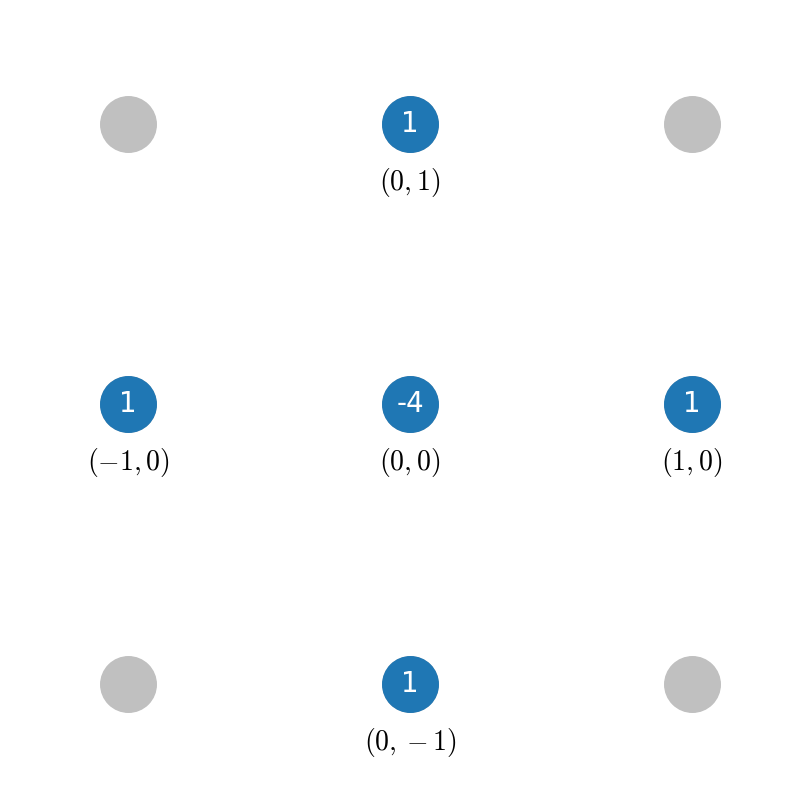
\includegraphics[width=0.3\textwidth]{diags/laplace2d.png}
    \caption{2D Laplacian Finite Difference Stencil}
\end{figure}

One has the option to craft these stencils as they see fit according to their training data.


\subsection{Convergence of Discrete Sobolev Norm}

% \begin{proposition}[Discrete Sobolev Norm Converges to Continuous Sobolev Norm]
%     Let \( f \in W^{p}_{r,s,\mathbf{h} }(Q^s) \) be a function in the discrete Sobolev space of dimension \( s \), order \( r \) and resolutions \(\mathbf{h} \) across its dimensions. The discrete Sobolev norm \( \| f \|_{W^{p}_{r,s}(Q^s)} \) converges to the continuous Sobolev norm \( \| f \|_{W^{p}_{r,s}} \) as \( \mathbf{h} \) increases.
% \end{proposition}

% \begin{proof}
%     This result is easily precipitated as one sees that for increasing \(\mathbf{h} \) our discrete derivatives converge to the continuous derivatives, and so the \(L^p\) norms of these derivatives converge to the continuous \(L^p\) norms. Taking the \(p\)th root and summing over all \( \mathbf{k} \leq r \) gives the discrete Sobolev norm, which in turn also converges to the continuous Sobolev norm.
% \end{proof}

\begin{proposition}[Discrete Sobolev Norm Converges to Continuous Sobolev Norm]
    

Consider a function \( u \in W^{k,p}(\Omega) \) and its approximations \( u_h \) defined on a mesh \( \Omega_h \). The mesh resolution increases as \( h \to 0 \). We aim to show that:
\[ \|u_h\|_{h,k,p} \to \|u\|_{W^{k,p}(\Omega)} \text{ as } h \to 0, \]
where \( \|u_h\|_{h,k,p} \) denotes the discrete Sobolev norm and \( \|u\|_{W^{k,p}(\Omega)} \) denotes the continuous Sobolev norm.

\end{proposition}

\begin{proof}

The discrete Sobolev space is defined by:
\[ W^{k,p}_h(\Omega_h) = \{ u_h \in l^p(\Omega_h) : D^\alpha_h u_h \in l^p(\Omega_h) \text{ for all } |\alpha| \leq k \}, \]
with the norm:
\[ \|u_h\|_{h,k,p} = \left( \sum_{|\alpha| \leq k} \|D^\alpha_h u_h\|_{l^p_h(\Omega_h)}^p \right)^{1/p}. \]

Assume \( u_h \) converges to \( u \) in \( L^p(\Omega) \) and \( D^\alpha_h u_h \) converges to \( D^\alpha u \) in \( L^p(\Omega) \) for all \( |\alpha| \leq k \). 

\paragraph*{Norm Convergence}
By the definitions of \( L^p \) norms and convergence assumptions:
\begin{align*}
\lim_{h \to 0} \|D^\alpha_h u_h\|_{l^p_h(\Omega_h)} &= \|D^\alpha u\|_{L^p(\Omega)}, \\
\lim_{h \to 0} \sum_{|\alpha| \leq k} \|D^\alpha_h u_h\|_{l^p_h(\Omega_h)}^p &= \sum_{|\alpha| \leq k} \|D^\alpha u\|_{L^p(\Omega)}^p.
\end{align*}

\paragraph*{Applying the Limit}
Taking the \( p \)-th root over the summation:
\[ \lim_{h \to 0} \|u_h\|_{h,k,p} = \left( \sum_{|\alpha| \leq k} \|D^\alpha u\|_{L^p(\Omega)}^p \right)^{1/p} = \|u\|_{W^{k,p}(\Omega)}. \]

\paragraph*{Conclusion}
Therefore, as \( h \) approaches zero, the discrete Sobolev norm of \( u_h \) converges to the continuous Sobolev norm of \( u \), verifying the efficacy of the mesh refinement in numerical approximations.

\end{proof}


\subsubsection{Speed of Convergence}

We examine now the speed of convergence of the discrete Sobolev norm as we have increasing dimensions.

\begin{figure}[h]
    \centering
    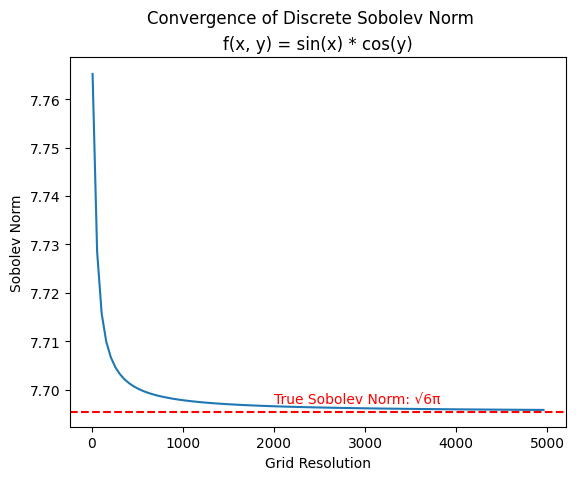
\includegraphics[width=0.6\textwidth]{diags/convergence.png}
    \caption{Convergence of the discrete Sobolev norm as \( \mathbf{h} \) increases, \(f \in W^{2}_{2,2}\) }
    \label{fig:convergence}
\end{figure}
\begin{figure}[h]
    \centering
    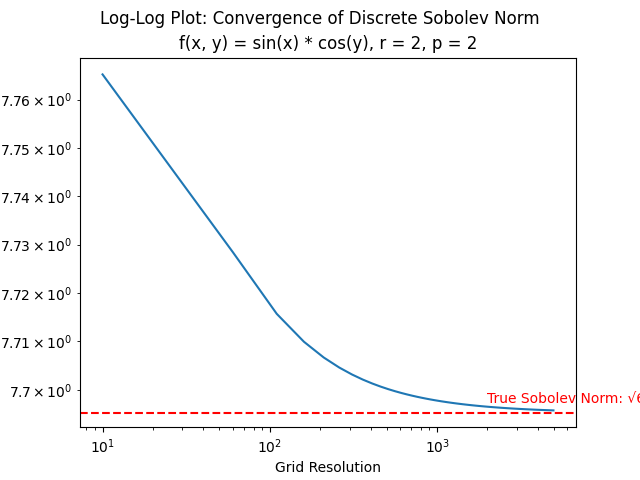
\includegraphics[width=0.6\textwidth]{diags/LogLog-Convergence.png}
    \caption{Convergence of the discrete Sobolev norm as \( \mathbf{h} \) increases, \(f \in W^{2}_{2,2}\) }
    \label{fig:convergence}
\end{figure}

\begin{figure}[h]
    \centering
    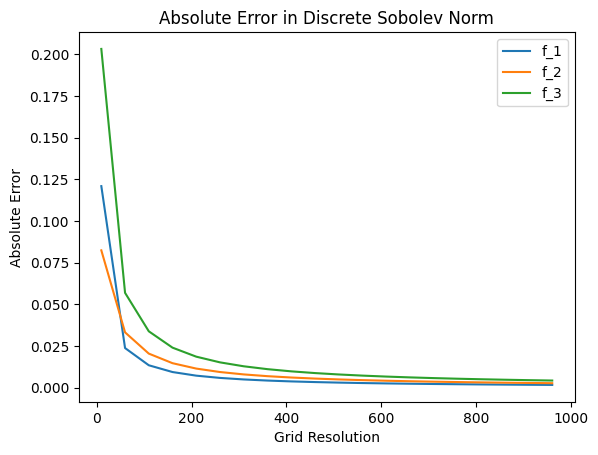
\includegraphics[width=0.6\textwidth]{diags/sob_dims.png}
    \caption{Convergence of the discrete Sobolev norm for \(f_{i}(\mathbf{x} ) = \prod_{x_{i}} \sin(x_{i}), i = 1,2,3\) }
    \label{fig:}
\end{figure}

\subsection{Order of Discrete Sobolev Norm}

We have now established that the discrete Sobolev norm converges to the continuous Sobolev norm as the resolution increases. We now examine how changing the order \(r\) of the discrete Sobolev norm affects its value.

There has been a change in premise from moving between continuous and discrete spaces. We no longer assume that our target function is in some Sobolev space, but rather assign our training data to some discrete Sobolev space. We have the choice of the order of the discrete Sobolev norm, and see if this aligns with the approximation results.

\begin{proposition}
    Let \( f \in W^{p}_{r,s} \) be a function in either the discrete Sobolev space or the continuous Sobolev space.
    Claim: the respective norm of the function is monotonically increasing in the order \( r \) of the Sobolev norm.
\end{proposition}
\begin{proof}
\begin{enumerate}
    \item \textbf{Norm Inclusion}: By definition, the norm \( \|u\|_{W^{k+1,p}(\Omega)} \) includes all the terms of \( \|u\|_{W^{k,p}(\Omega)} \) plus additional terms for the derivatives of order \( k+1 \). Specifically:
    \[
    \|u\|_{W^{k+1,p}(\Omega)}^p = \|u\|_{W^{k,p}(\Omega)}^p + \sum_{|\alpha| = k+1} \|D^\alpha u\|_{L^p(\Omega)}^p.
    \]

    \item \textbf{Non-Negativity of \( L^p \) Norms}: Since the \( L^p \) norms of the derivatives \( \|D^\alpha u\|_{L^p(\Omega)} \) are non-negative, the sum of these norms is also non-negative.

    \item \textbf{Monotonic Increase}: This leads directly to the inequality:
    \[
    \| u\|_{W^{k+1,p}(\Omega)}^p \geq \|u\|_{W^{k,p}(\Omega)}^p
    \]
\end{enumerate}
\end{proof}

\begin{figure}[h]
    \centering
    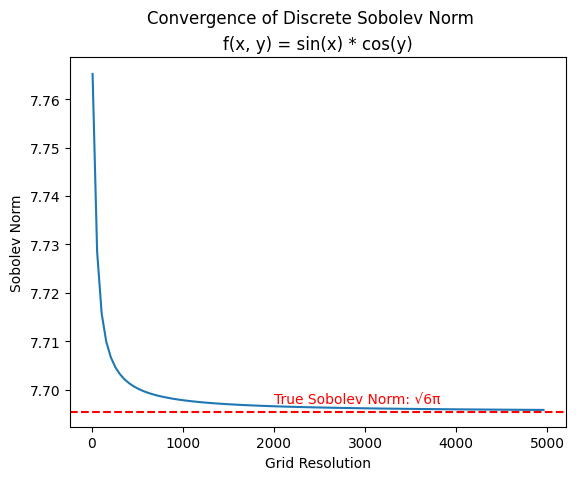
\includegraphics[width=0.5\textwidth]{diags/convergence.png}
    \caption{Convergence of Discrete Sobolev Norm for \(f \in W^{2}_{2,2}\) }
    \label{fig:order}
\end{figure}
\begin{figure}[h]
    \centering
    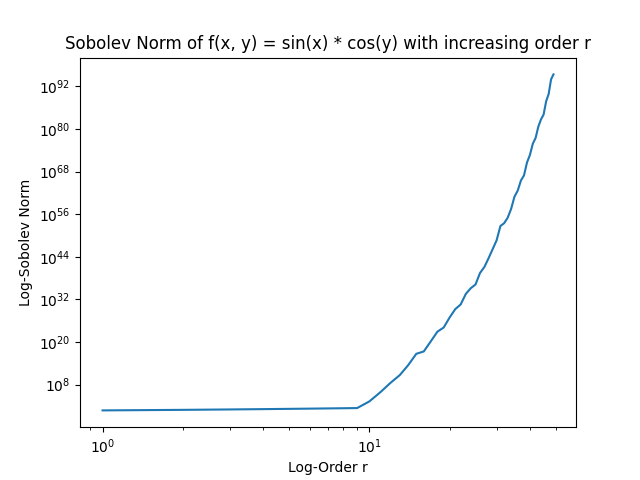
\includegraphics[width=0.5\textwidth]{diags/SobolevNormIncreasingOrder.png}
    \caption{Discrete Sobolev Norm for increasing order for \(f \in W^{2}_{r,2}\) }
    \label{fig:order}
\end{figure}

This result is key, as it tells us that for some functions, say for example those with unbounded derivatives at some point, the discrete Sobolev norm may explode. In relation to the inequality;

    \[ \left\|f - \sum_{j=1}^{n} a_j(f) \phi(A_j(\cdot) + b)\right\|_p \leq c n^{-r/s} \|f\|_{W^p_{r,s}} \]

we see that by having training data in some higher order discrete Sobolev space, we may find that the dominating term in the right hand of the equality is the discrete Sobolev norm, and so the approximation results may not hold for large \(r\), i.e. functions assumed to be very smooth.

\end{document}

